\section{Penjelasan Regresi Linier Serderhana}
\par Regresi Linear Sederhana adalah Metode Statistik yang berfungsi untuk menguji sejauh mana hubungan sebab akibat antara Variabel Faktor Penyebab (X) terhadap Variabel Akibatnya. Faktor Penyebab pada umumnya dilambangkan dengan X atau disebut juga dengan Predictor sedangkan Variabel Akibat dilambangkan dengan Y atau disebut juga dengan Response. Regresi Linear Sederhana atau sering disingkat dengan SLR (Simple Linear Regression) juga merupakan salah satu Metode Statistik yang dipergunakan dalam produksi untuk melakukan peramalan ataupun prediksi tentang karakteristik kualitas maupun Kuantitas.
\par Contoh Penggunaan Analisis Regresi Linear Sederhana dalam Produksi antara lain :
\begin{enumerate}
    \item Hubungan antara Lamanya Kerusakan Mesin dengan Kualitas Produk yang dihasilkan.
    \item Hubungan Jumlah Pekerja dengan Output yang diproduksi.
    \item Hubungan antara suhu ruangan dengan Cacat Produksi yang dihasilkan.
\end{enumerate}
\par Model Persamaan Regresi Linear Sederhana adalah seperti berikut ini : Y = a + bX
\par Dimana :
\par Y = Variabel Response atau Variabel Akibat (Dependent)
\par X = Variabel Predictor atau Variabel Faktor Penyebab (Independent)
\par a = konstanta
\par b = koefisien regresi (kemiringan); besaran Response yang ditimbulkan oleh Predictor.
\par Nilai-nilai a dan b dapat dihitung dengan menggunakan Rumus dibawah ini :
\par a =   ((Σy) (Σx²) – (Σx) (Σxy)) / n(Σx²) – (Σx)²
\par b =   (n(Σxy) – (Σx) (Σy)) / n(Σx²) – (Σx)²
\par Berikut ini adalah Langkah-langkah dalam melakukan Analisis Regresi Linear Sederhana :
\begin{enumerate}
    \item Tentukan Tujuan dari melakukan Analisis Regresi Linear Sederhana 
    \item Identifikasikan Variabel Faktor Penyebab (Predictor) dan Variabel Akibat (Response)
    \item Lakukan Pengumpulan Data
    \item Hitung  X², Y², XY dan total dari masing-masingnya
    \item Hitung a dan b berdasarkan rumus diatas.
    \item Buatkan Model Persamaan Regresi Linear Sederhana.
    \item Lakukan Prediksi atau Peramalan terhadap Variabel Faktor Penyebab atau Variabel Akibat.
\end{enumerate}
\section {Contoh Kasus Regresi Linier Sederhana dan Penyelesaiannya}
\section {Contoh Kasus Regresi Linier Sederhana dan Hasilnya}

\section{Penjelasan Regresi Linier Berganda}
\par Dalam suatu penelitian, pada beberapa kenyataan akan ada lebih dari satu variabel independen yang mempengaruhi variabel dependen yang kita inginkan. Misalnya, keadaan dimana kemampuan komunikasi adalah variabel yang mempengaruhi nilai prestasi kerja. Keadaan demikian kelihatannya sangat tidak realistik. Kenyataannya, yang mempengaruhi prestasi kerja tidak hanya kemampuan komunikasi namun dapat pula dilihat misalnya dari kemampuan bekerjasama, kemampuan IT, kemampuan berbahasa inggrisnya dan lainnya. Untuk menganalisis beberapa variabel yang mempengaruhi satu variabel lain maka kita menggunakan analisis regresi linear berganda.      
\par Regresi pertama-tama dipergunakan sebagai konsep statistik pada tahun 1877 oleh Sir Francis Galton, seorang ilmuwan asal Inggris yang melakukan studi tentang kecenderungan tinggi badan anak. Hasil studi tersebut memberikan suatu kesimpulan bahwa kecenderungan tinggi badan anak yang lahir terhadap orangtuanya adalah menurun (regress) mengarah pada tinggi badan rata-rata penduduk. Istilah regresi pada mulanya bertujuan untuk membuat perkiraan nilai satu variabel (tinggi badan anak) terhadap satu variabel yang lain (tinggi badan orangtua). Selanjutnya berkembang menjadi alat untuk membuat perkiraan nilai suatu variabel dengan menggunakan beberapa variabel lain yang berhubungan dengan variabel tersebut. 
\section{Pengertian Regresi Linier Berganda}
\par Regresi linear adalah alat statistik yang dipergunakan untuk mengetahui pengaruh antara satu atau beberapa variabel terhadap satu buah variabel. Variabel “penyebab” atau yang dikenal sebagai variabel yang mempengaruhi disebut dengan bermacammacam istilah: variabel independen, variabel bebas, variabel penjelas, variabel eksplanatorik, atau variabel X (karena seringkali digambarkan dalam grafik sebagai absis, atau sumbu X). Sedangkan, variabel “akibat” dikenal sebagai variabel yang dipengaruhi, variabel dependen, variabel terikat, atau variabel Y. Secara umum, persamaan regresi dapat terdiri dari satu atau lebih peubah bebas namun hanya memiliki satu peubah terikat. Dari contoh sebelumnya, mengikuti bimbingan belajar dan belajar mandiri sebagai variabel yang mempengaruhi (X) adalah, sedangkan nilai prestasi siswa sebagai variabel yang dipengaruhi.  
\par Analisis regresi membentuk persamaan garis lurus (linear) dan menggunakan persamaan tersebut untuk membuat perkiraan (prediction). Berdasarkan jumlah variabel bebas, analisis regresi linear yang terdiri dari dua variabel dikenal dengan analisis linear sederhana, sedangkan yang lebih dari dua variabel disebut analisis linear berganda dan yang akan kita pelajari lebih lanjut.  
\par Tujuan dari analisis regresi yaitu pertama untuk membuat perkiraan nilai suatu variabel terikat jika nilai variabel bebas yang berhubungan dengannya sudah ditentukan dan yang kedua untuk menguji hipotesis signifikansi pengaruh dari variabel bebas terhadap variabel terikat.  
\par Model regresi linier berganda untuk dua variabel bebas dan satu variabel terikat adalah sebagai berikut: 
\begin{figure}[ht]
\centering
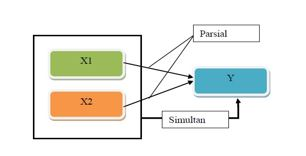
\includegraphics[width=7cm, height=5cm]{figures/modelregresi.JPG}
\caption{\textit{Model Regresi Linier Berganda}
\label{eq:31}}
\end{figure} 
\par Model diatas dapat dijelaskan bahwa dalam model regresi linier berganda mempunyai dua uji pengaruh yaitu :  
\begin{enumerate}
\item 	Pengaruh variabel X (bebas) secara simultan terhadap variabel Y (terikat)  
\item 	Pengaruh variabel X (bebas) secara parsial terhadap variabel Y (terikat), yaitu meliputi:  
\end{enumerate}
    \begin{itemize}
               \item Pengaruh variabel X1 terhadap variabel Y  
               \item Pengaruh variabel X2 terhadap variabel Y 
               \end{itemize}
\section{Tujuan Regresi Linier Berganda}
\begin{enumerate}
\item Untuk membuat perkiraan nilai suatu variabel terikat jika nilai variabel bebas yang berhubungan dengannya sudah ditentukan
\item Untuk menguji hipotesis signifikansi pengaruh dari variabel bebas terhadap variabel terikat
\end{enumerate}

\section{Manfaat Regresi Linier Berganda}
\begin{enumerate}
\item Model regresi dapat digunakan untuk mengukur keeratan hubungan antara variabel dependen (tak bebas) dan variabel independen (bebas). 
\item Model regresi dapat digunakan untuk mengetahui pengaruh suatu atau beberapa variabel independen terhadap variabel dependen (respons).
\item Model regresi dapat digunakan untuk mengetahui pengaruh suatu atau beberapa variabel independen terhadap variabel dependen (respons).
\end{enumerate}

\section{Kelebihan Dan Kekurangan Regresi Linier Berganda}
\par Kelebihan : Dengan menggunakan regresi linear berganda maka dapat menganalisis dengan menggunakan beberapa variabel bebas (X) sehingga hasil prediksi yang didapatkan lebih akurat dibandingkan dengan regresi linear sederhana yang hanya menggunakan satu variabel bebas (X). 
\par Kekurangan : Tidak mampu menunjukkan titik jenuh fungsi yang sedang diselidiki akibatnya selalu timbul kemungkinan kesalahan prediski dan Terdapat kemungkinan terjadinya multikolinearitas pada variabel-variabel bebas. Akibatnya variabel bebas tidak mampu menjelaskan variabel tak bebas (hubungan antara X dan Y tidak bermakna).
\section{Rumus Metode Regresi Linear Berganda}

Analisis regresi linier berganda adalah hubungan secara linear antara dua atau lebih variabel independen (X1, X2) dengan variabel dependen (Y). Analisis ini untuk mengetahui arah hubungan antara variabel independen dengan variabel dependen apakah masing-masing variabel independen berhubungan positif atau negatif dan untuk memprediksi nilai dari variabel dependen apabila nilai variabel independen mengalami kenaikan atau penurunan. Data yang digunakan biasanya berskala interval atau rasio\citep{smadi2012least}.
Persamaan regresi linear berganda sebagai berikut:
\begin{equation}
        Y= a+b_{1}X_{1}+b_{2}X_{2}...+b_{n}X_{n}
    \end{equation}
Keterangan:
\par Y’                    =   Variabel dependen (nilai yang diprediksikan)
\par X1 dan X2      =   Variabel independen
\par a                      =   Konstanta (nilai Y’ apabila X1, X2…..Xn = 0)
\par b                            =    Koefisien regresi (nilai peningkatan ataupun penurunan)
\section{Contoh soal Cara Kerja Metode Regresi Linear}
\subsection{Contoh soal 1}
\par Di contoh soal pertama ini penulisa mengambil permasalahan dari kasus di PT Pertamina Gas. Pada kasus di penelitian ini penulis melakukan prediksi \textit{reveniew} dari 5 wilayah milik PT Pertamina Gas. Dan dari setiap wilayah tersebut ada \textit{shipper}(sumber) dan \textit{offtaker}(konsumen)
	Y adalah variabel terikat yang diramalkan (shipper), X adalah variabel bebas. nilai x1(offtaker sinngle) nilai x2 (nilai offtaker multi)\citep{hijriani2017implementasi}
Berikut ini adalah Langkah-langkah dalam melakukan prediksi Regresi Linear Berganda:\citep{analisisrls}
\begin{enumerate}
        \item 	Tentukan nilai a dan b dengan menggunakan SPSS dari 5 wilayah pada PT Pertamina Gas yang di ambil dari data total shipper dan offtaker dari bulan sebelumnya.
\begin{table}[!ht]
\centering
\caption{\textbf{Eastern Java Area}}
\begin{tabular}{|c|c|c|c|}
\hline
Minggu & Shipper & Single & Multi \\ \hline
1      & 965     & 15     & 308   \\ \hline
2      & 910     & 34     & 616   \\ \hline
3      & 944     & 27     & 616   \\ \hline
4      & 932     & 26     & 637   \\ \hline
5      & 267     & 10     & 183   \\ \hline
\end{tabular}
\end{table}
\begin{lstlisting}
a= Y-b1X1-b2X2      
a= 325.069
\end{lstlisting}
\begin{figure}[!ht]
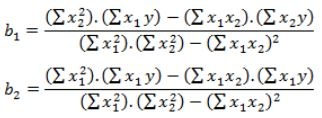
\includegraphics[scale=0.6]{figures/b1b2.JPG}
\label{Figure4}
\end{figure}
\begin{lstlisting}
b1= -4.545
b2= 1.23
Rumus:
Y= a+b1X1+b2X2
Y= 325.069+(-4.545x1)+1.23X2
\end{lstlisting}

\begin{table}[!ht]
  \centering
  \caption{\textbf{Kalimantan Area}}
\begin{tabular}{|c|c|c|c|}
\hline
Minggu & Shipper & Single & Multi \\ \hline
1      & 560     & 21     & 378   \\ \hline
2      & 630     & 7     & 378   \\ \hline
3      & 560     & 21     & 378   \\ \hline
4      & 560     & 21     & 378   \\ \hline
5      & 180     & 2     & 108   \\ \hline
\end{tabular}
\end{table}
\begin{lstlisting}
a= Y-b1X1-b2X2      
a= -0.00000000000014
\end{lstlisting}
\begin{figure}[!ht]
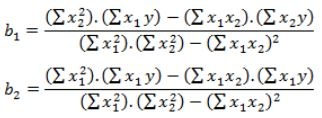
\includegraphics[scale=0.6]{figures/b1b2.JPG}
    \label{Figure4}
\end{figure}
\begin{lstlisting}
b1= -5
b2= 1.759
Rumus:
Y= a+b1X1+b2X2
Y= -0.00000000000014+(-5x1)+1.759X2
\end{lstlisting}

\begin{table}[!ht]
 \centering
  \caption{\textbf{Northem Sumatra Area}}
\begin{tabular}{|c|c|c|c|}
\hline
Minggu & Shipper & Single & Multi \\ \hline
1      & 597     & 20     & 444   \\ \hline
2      & 646     & 70     & 378   \\ \hline
3      & 737     & 62.01     & 386   \\ \hline
4      & 700     & 70     & 386   \\ \hline
5      & 200     & 20     & 108   \\ \hline
\end{tabular}
\end{table}
\newpage \begin{lstlisting}
a= Y-b1X1-b2X2      
a= 3.319
\end{lstlisting}
\begin{figure}[!htbp]
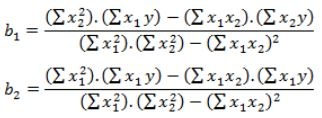
\includegraphics[scale=0.6]{figures/b1b2.JPG}
    \label{Figure4}
\end{figure}
\begin{lstlisting}
b1= 3.342
b2= 1.207
Rumus:
Y= a+b1X1+b2X2
Y= 3.319+3.342x1+1.207X2
\end{lstlisting}

\begin{table}[!ht]
  \centering
  \caption{\textbf{Southern Sumatra Area}}
\begin{tabular}{|c|c|c|c|}
\hline
Minggu & Shipper & Single & Multi \\ \hline
1      & 640.43     & 9     & 378   \\ \hline
2      & 665.96     & 8     & 378   \\ \hline
3      & 630     & 13     & 378   \\ \hline
4      & 630     & 9     & 378   \\ \hline
5      & 180     & 2     & 108   \\ \hline
\end{tabular}
\end{table}
\begin{lstlisting}
a= Y-b1X1-b2X2      
a= -9.915
\end{lstlisting}
\begin{figure}[!ht]
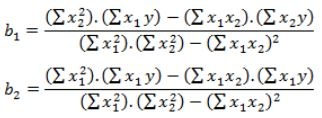
\includegraphics[scale=0.6]{figures/b1b2.JPG}
    \label{Figure4}
\end{figure}
\begin{lstlisting}
b1= -4.797
b2= 1.847
Rumus:
Y= a+b1X1+b2X2
Y= -9.915+(-4.797x1)+1.847X2
\end{lstlisting}

\begin{table}[!ht]
 \centering
  \caption{\textbf{Western Java Area}}
\begin{tabular}{|c|c|c|c|}
\hline
Minggu & Shipper & Single & Multi \\ \hline
1      & 630     & 14    & 315   \\ \hline
2      & 700     & 14    & 313   \\ \hline
3      & 700     & 14     & 308   \\ \hline
4      & 700     & 14     & 353   \\ \hline
5      & 200     & 4     & 133   \\ \hline
\end{tabular}
\end{table}
\newpage \begin{lstlisting}
a= Y-b1X1-b2X2      
a= -15.599
\end{lstlisting}
\begin{figure}[!htbp]
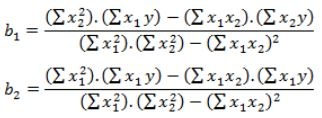
\includegraphics[scale=0.6]{figures/b1b2.JPG}
    \label{Figure4}
\end{figure}
\begin{lstlisting}
b1= 40.786
b2= 0.394
Rumus:
Y= a+b1X1+b2X2
Y= -15.599+40.786x1+0.394X2
\end{lstlisting}
\item Setelah itu masukkan ke rumus untuk memprediksi nilai Y(shipper). Y= a+b1X1+b2X2
\item Setelah nilai Y di temukan di kurangkan kembali dengan nilai total perminggu offtaker single dan multi untuk mengetahui sisa shipper.
\item Setelah di temukan nilai total pendapatan perminggu kemudian di jumlahkan untuk mengetahui total pendapatan perbulan
\item Untuk mengetahui reveniew nya total perbulan di akumulasikan ke dollar (perkalian 1MSCF= 4 US dollar).
\end{enumerate}
\subsection{Contoh soal 2}
\par Kita mengambil contoh kasus pada uji normalitas, yaitu sebagai berikut: Seorang mahasiswa bernama Bambang melakukan penelitian tentang faktor-faktor yang mempengaruhi harga saham pada perusahaan di BEJ.\citep{priyatno2014spss} Bambang dalam penelitiannya ingin mengetahui hubungan antara rasio keuangan PER dan ROI terhadap harga saham. Dengan ini Bambang menganalisis dengan bantuan program SPSS dengan alat analisis regresi linear berganda. Dari uraian di atas maka didapat variabel dependen (Y) adalah harga saham, sedangkan variabel independen (X1 dan X2) adalah PER dan ROI.
Data-data yang di dapat berupa data rasio dan ditabulasikan sebagai berikut: \begin{figure}[!htbp]
    \centering
    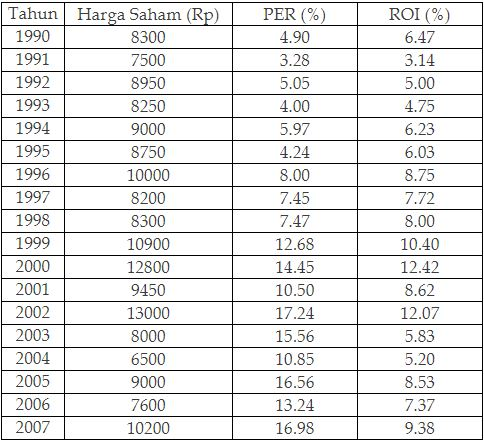
\includegraphics[scale=0.7]{figures/cs.JPG}
    \caption{Tabulasi Data (Data Fiktif)}
\end{figure}
\newpage \par Langkah berikutnya sama dengan langkah di contoh soal 1. Mencari nilai a dan b nya. \begin{lstlisting}
a= Y-b1X1-b2X2      
a= 4662.491
\end{lstlisting}
\begin{figure}[!htbp]
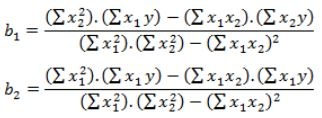
\includegraphics[scale=0.6]{figures/b1b2.JPG}
    \label{Figure4}
\end{figure}
\begin{lstlisting}
b1= -74.482
b2= 692.107
\end{lstlisting}
Setelah variabel a dan b di temukan maka di masukkan ke dalam rumus seperti berikut: 
Persamaan regresinya sebagai berikut:
\begin{lstlisting}
Y’ = a + b1X1+ b2X2
Y’ =  4662,491 + (-74,482)X1 + 692,107X2
Y’ =  4662,491 - 74,482X1 + 692,107X2
\end{lstlisting}
Keterangan:
\begin{lstlisting}
Y’        = Harga saham yang diprediksi (Rp)
a          = konstanta
b1,b2    = koefisien regresi
X1        = PER (\%)
X2        = ROI (\%)
\end{lstlisting}
\par Langkah berikutnya adalah memasukkan nilai x1(PER (\%)) dan x2(ROI (\%)) ke dalam rumus, sehingga di temukan hasil prediksi sebagai berikut:
\begin{figure}[!htbp]
    \centering
    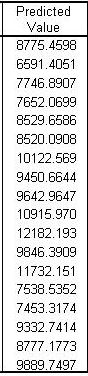
\includegraphics[scale=0.6]{figures/cs3.JPG}
    \caption{Hasil Perhitungan Prediksi}
\end{figure}
\subsection{Contoh soal 3}
\par Di contoh soal 3 ini kita akan menghitung data pengeluaran 10 rumah tangga, untuk pembelian barang tahan lama per minggu(Y), pendapatan per minggu (X1), dan jumlah anggota keluarga (X2).
\par Berikut adalah data mentahan nya:
\begin{figure}[!htbp]
    \centering
    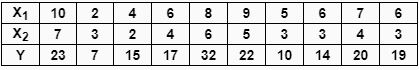
\includegraphics[scale=0.7]{figures/css.JPG}
    \caption{Data mentahan}
\end{figure}
